\newcommand{\defs}{../defs}
\documentclass[usenames,dvipsnames]{beamer}

\usepackage[brazilian]{babel}
\usepackage[utf8]{inputenc}
\usepackage{ragged2e}
\usepackage{etoolbox}
\usepackage{multirow}
\usepackage{natbib}
\usepackage{subfigure}
\usepackage{caption}
\usepackage{tikz}
\usepackage{amsmath}
\usepackage{amssymb}
\usepackage{adjustbox}
\usepackage{booktabs}
\usepackage{array}
\usepackage{dot2texi}
\usepackage{minted}
\usepackage{mdframed}
\usepackage{ragged2e}
\usepackage[ruled,vlined]{algorithm2e}

\usefonttheme[onlymath]{serif}

\renewcommand{\thealgocf}{}

\usetheme{Boadilla}
\usecolortheme{seahorse}

\author[Prof. Marcelo de Souza]{}
\date[Udesc Ibirama]{}

\renewcommand{\maketitle}{
	\frame[plain]{
		\titlepage
		\centering
		
		{\scriptsize
			\begin{tikzpicture}[remember picture,overlay,shift={(current page.center)}]
			\node at (-5.7,-4.13) {
\includegraphics[width=.2\textwidth,trim={0 19cm 0 0},clip]{\defs/img/logo-udesc.pdf}};
			\node[align=center]  at (0,-0.4) {%
				\small\textbf{Prof. Marcelo de Souza}\\[3pt]
				\small\texttt{marcelo.desouza@udesc.br}
			};
			\end{tikzpicture}
		}
		
		{\scriptsize
			\begin{tikzpicture}[remember picture,overlay,shift={(current page.center)}]
			\node at (-5.7,-4.13) {
\includegraphics[width=.2\textwidth,trim={0 19cm 0 0},clip]{\defs/img/logo-udesc.pdf}};
			\node[align=left] at (-2.4,-4.11) {%
				\color{black!80}Algoritmos e Estruturas de Dados\\
				\color{black!80}Bacharelado em Engenharia de Software\\
				\color{black!80}Universidade do Estado de Santa Catarina%
			};
			\end{tikzpicture}
		}
	}
}

\addtobeamertemplate{frametitle}{}{%
	\begin{tikzpicture}[remember picture,overlay]
		\node[anchor=north east,xshift=12pt,yshift=2pt] at (current page.north east){
			
\includegraphics[height=1cm,trim={0 19cm 0 0},clip]{\defs/img/logo-udesc.pdf}
		};
	\end{tikzpicture}
}

\addtobeamertemplate{frametitle}{}{\vspace*{-0.5cm}}

\renewcommand{\familydefault}{\sfdefault}

\colorlet{codeboxcolor}{blue!8}

\surroundwithmdframed{minted}

\BeforeBeginEnvironment{mdframed}{}
\AfterEndEnvironment{mdframed}{}

\mdfsetup{%
	backgroundcolor=codeboxcolor,
	linecolor=white}

\setminted{%
	mathescape,
	escapeinside=@@,
	linenos,
	breaklines,
	tabsize=3,
	fontsize=\footnotesize}

\def\arraystretch{1.5}

\captionsetup[figure]{labelformat=empty}
\captionsetup[table]{labelformat=empty}

%\setbeamercovered{transparent}
\setbeamercovered{invisible}

\definecolor{black}{RGB}{0, 0, 0}
\definecolor{darkred}{RGB}{179, 0, 0}
\definecolor{darkblue}{RGB}{0, 0, 51}

\setbeamertemplate{itemize item}{\footnotesize\raise1.25pt\hbox{\color{darkred}$\bullet$}}
\setbeamertemplate{itemize subitem}{\scriptsize\raise1pt\hbox{\color{darkred}$\circ$}}
\setbeamertemplate{itemize subsubitem}{\scriptsize\raise1.5pt\hbox{\color{darkred}$\triangleright$}}
\setbeamertemplate{enumerate item}{\color{darkred}\insertenumlabel.}
\setbeamertemplate{enumerate subitem}{\color{darkred}\insertenumlabel.\insertsubenumlabel}
\setbeamertemplate{enumerate subsubitem}{\color{darkred}\insertenumlabel.\insertsubenumlabel.\insertsubsubenumlabel}

\AtBeginEnvironment{block}{
	\setbeamertemplate{itemize item}{\footnotesize\raise1.25pt\hbox{\color{black}$\bullet$}}
	\setbeamertemplate{itemize subitem}{\scriptsize\raise1pt\hbox{\color{black}$\circ$}}
	\setbeamertemplate{itemize subsubitem}{\scriptsize\raise1.5pt\hbox{\color{black}$\triangleright$}}
	\setbeamertemplate{enumerate item}{\color{black}\insertenumlabel.}
	\setbeamertemplate{enumerate subitem}{\color{black}\insertenumlabel.\insertsubenumlabel}
	\setbeamertemplate{enumerate subsubitem}{\color{black}\insertenumlabel.\insertsubenumlabel.\insertsubsubenumlabel}
}
\AtBeginEnvironment{exampleblock}{
	\setbeamertemplate{itemize item}{\footnotesize\raise1.25pt\hbox{\color{black}$\bullet$}}
	\setbeamertemplate{itemize subitem}{\scriptsize\raise1pt\hbox{\color{black}$\circ$}}
	\setbeamertemplate{itemize subsubitem}{\scriptsize\raise1.5pt\hbox{\color{black}$\triangleright$}}
	\setbeamertemplate{enumerate item}{\color{black}\insertenumlabel.}
	\setbeamertemplate{enumerate subitem}{\color{black}\insertenumlabel.\insertsubenumlabel}
	\setbeamertemplate{enumerate subsubitem}{\color{black}\insertenumlabel.\insertsubenumlabel.\insertsubsubenumlabel}
}

\AtBeginEnvironment{alertblock}{
	\setbeamertemplate{itemize item}{\footnotesize\raise1.25pt\hbox{\color{black}$\bullet$}}
	\setbeamertemplate{itemize subitem}{\scriptsize\raise1pt\hbox{\color{black}$\circ$}}
	\setbeamertemplate{itemize subsubitem}{\scriptsize\raise1.5pt\hbox{\color{black}$\triangleright$}}
	\setbeamertemplate{enumerate item}{\color{black}\insertenumlabel.}
	\setbeamertemplate{enumerate subitem}{\color{black}\insertenumlabel.\insertsubenumlabel}
	\setbeamertemplate{enumerate subsubitem}{\color{black}\insertenumlabel.\insertsubenumlabel.\insertsubsubenumlabel}
}

\let\oldenum\enumerate
\renewcommand\enumerate{\oldenum\justifying}

\let\olditem\itemize
\renewcommand\itemize{\olditem\justifying}

\setbeamertemplate{section in toc}{\color{darkred}\inserttocsectionnumber.~\color{black}\inserttocsection}

\setbeamertemplate{title page}[default][colsep=-4bp,rounded=true]

\setbeamercolor{frametitle}{bg=white}
\setbeamercolor{title}{bg=white}

\setbeamercolor{palette primary}{fg=darkred}
\setbeamercolor{palette secondary}{fg=darkblue}
\setbeamercolor{palette tertiary}{fg=darkblue}
\setbeamercolor{palette quaternary}{fg=darkblue}
\setbeamercolor{normal text}{fg=darkblue}

\setbeamerfont{frametitle}{size=\LARGE}
\setbeamerfont{title}{size=\LARGE}


\setbeamertemplate{footline}
{
	\leavevmode%
	\hbox{%
		\begin{beamercolorbox}[wd=.9\paperwidth,ht=2.25ex,dp=1ex,center]{}%
			\color{black!80} \hypersetup{hidelinks}%
			\insertshortauthor%
			\hspace*{4ex}%
			$\diamond$%
			\hspace*{4ex}%
			\insertshorttitle%
			\hspace*{4ex}%
			$\diamond$%
			\hspace*{4ex}%
			\insertshortdate%
		\end{beamercolorbox}%
		\begin{beamercolorbox}[wd=.1\paperwidth,ht=2.25ex,dp=1ex,right]{}%
			\color{black!80}
			\insertframenumber{} / \inserttotalframenumber\hspace*{2ex}
	\end{beamercolorbox}}%
	\vskip0pt%
}

\setbeamertemplate{navigation symbols}{}

\hypersetup{
	colorlinks,
	linkcolor={black},
	citecolor={blue!80!black},
	urlcolor={blue!80!black}
}

\usetikzlibrary{shapes,arrows,arrows.meta,chains,decorations.pathreplacing,automata,positioning}

\title[Árvore geradora mínima]{Árvore geradora mínima}
\subtitle{Algoritmos de Prim, Kruskal e Delete-Reverse}

\begin{document}

\maketitle

\begin{frame}{Material de consulta}
	\textbf{Leitura obrigatória:}
	\begin{itemize}
		\item Capítulo 3 de~\cite{Goldbarg2AndGoldbarg2012} -- Árvores.
		\item Capítulo 4 de~\cite{KleinbergAndTardos2006} -- Algoritmos gulosos.
	\end{itemize}
	
	\bigskip
	
	\textbf{Leitura complementar:}
	\begin{itemize}
		\item Capítulo 14 de~\cite{GoodrichEtAl2014} -- Algoritmos em grafos.
		\item Capítulo 15 de~\cite{Preiss2001} -- Grafos e algoritmos em grafos.
	\end{itemize}
\end{frame}


\begin{frame}{Árvore geradora}
	\framesubtitle{Conceitos}
	
	\begin{itemize}
		\item Uma {\color{magenta}árvore geradora} de um grafo $G = (V, E)$ é um subgrafo de $G$ que é acíclico (árvore) e conexo.
		\begin{itemize}
			\item Também chamada de \textit{árvore de cobertura} ou \textit{árvore de extensão}.
		\end{itemize}
	\end{itemize}

	\begin{figure}
		\centering
		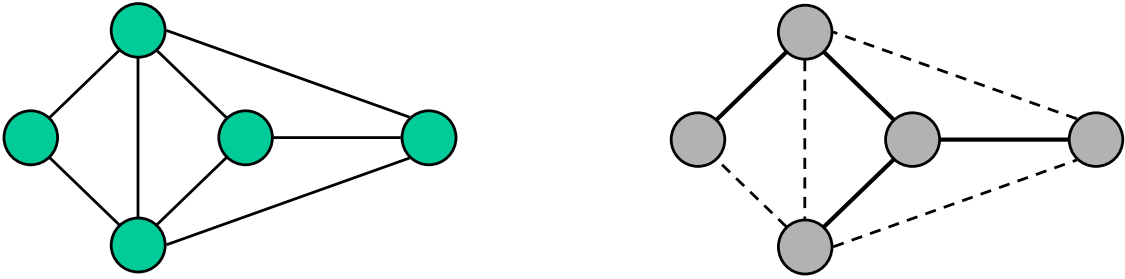
\includegraphics[width=0.9\linewidth]{img/arvore-geradora}
	\end{figure}
	
	\pause
	
	\begin{itemize}
		\item Se $T$ é uma árvore geradora de $G$, então:
		\begin{itemize}
			\item $T$ é acíclico e conectado.
			\item $T$ possui $n - 1$ arestas.
			\item Removendo uma aresta de $T$ torna o grafo desconexo.
			\item Inserindo uma aresta a $T$ torna o grafo cíclico.
		\end{itemize}
	\end{itemize}
\end{frame}



\begin{frame}{Árvore geradora mínima}
	\framesubtitle{Conceitos}
	
	\begin{itemize}
		\item Dado um grafo $G = (V, E)$ ponderado, uma {\color{magenta}árvore geradora mínima} é uma árvore geradora cujo somatório dos pesos das arestas é mínimo.
	\end{itemize}

	\begin{figure}
		\centering
		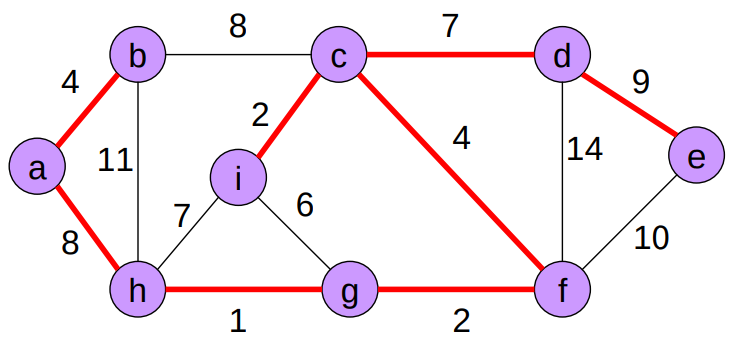
\includegraphics[width=0.55\linewidth]{img/arvore-cobertura-minima}
	\end{figure}
\end{frame}



\begin{frame}{Árvore geradora mínima}
	\framesubtitle{Aplicações}
	
	\begin{itemize}
		\item {\color{magenta}Cenário 1:} os pinos de uma placa de circuito impresso devem ser conectados com a menor quantidade de fio.
		\begin{itemize}
			\item Pinos são os vértices e os fios são as arestas.
		\end{itemize}
		
		\item {\color{magenta}Cenário 2:} a universidade deseja construir passarelas para ligar os prédios do campus. Quais passarelas devem ser construídas para termos o menor gasto possível de recusros financeiros?
		\begin{itemize}
			\item Prédios são os vértices e suas possíveis ligações são as arestas.
		\end{itemize}
		
		\item {\color{magenta}Cenário 3:} reconhecimento de faces em tempo real.
	\end{itemize}
	
	\begin{figure}
		\centering
		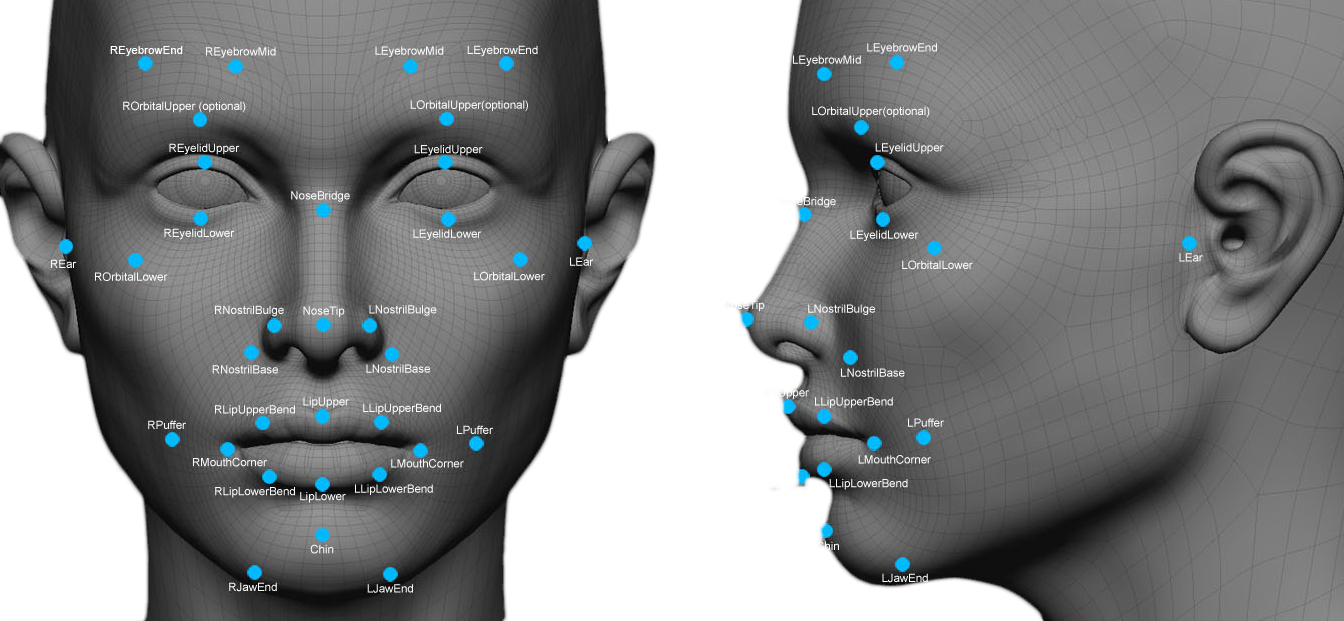
\includegraphics[width=0.55\linewidth]{img/face-recognition}
	\end{figure}
\end{frame}



\begin{frame}{Árvore geradora mínima}
	\framesubtitle{Algoritmos}
	
	\begin{itemize}
		\item \textbf{Problema:} dado um grafo conexo não-direcionado ponderado $G = (V, E)$, encontra uma árvore geradora mínima $H = (G, T)$.
		
		\medskip
		
		\pause
		
		\item {\color{magenta}Algoritmo de Prim:} análogo ao algoritmo de Dijkstra, inicia de um vértice raiz $s$ e cresce uma árvore a partir dele. A cada iteração insere o vértice que pode ser alcançado com menor custo a partir da árvore parcialmente construída.
		
		\pause
		
		\item {\color{magenta}Algoritmo de Kruskal:} inicia a árvore sem nenhuma aresta (somente os vértices). Iterativamente insere arestas de $E$, do menor ao maior custo, desde que sua inserção não forme um ciclo em $H$.
		
		\pause
		
		\item {\color{magenta}Algoritmo Reverse-Delete:} é a versão reversa do algoritmo de Kruskal. Inicia com $H = V$ e, iterativamente, remove arestas do maior para o menor custo, desde que a remoção não desconecte o grafo.
	\end{itemize}
\end{frame}



\begin{frame}{Algoritmo de Prim}
	\framesubtitle{Pseudocódigo}
	
	\begin{algorithm}[H]
		\DontPrintSemicolon
		
		$Q \gets V$\;
		Set $d(v) = \infty$ and $p(v) = -1$ for each $v \in V$\;
		$d(s) = 0$\;
		
		\While{$Q \neq \emptyset$}{
			$u \gets$ extract-min($Q$)\;
			\For{each $v$ adjacent to $u$}{
				\If{$v \in Q$ and $d(v) > w(u, v)$}{
					$d(v) \gets w(u, v)$\;
					$p(v) \gets u$\;
					update($Q, v$)\;
				}
			}
		}
		
		\caption{\texttt{prim(Vertex s)}}
	\end{algorithm}
\end{frame}



\begin{frame}{Algoritmo de Prim}
	\framesubtitle{Funcionamento}
	
	\begin{itemize}
		\item Uma execução intermediária do algoritmo de Prim:
	\end{itemize}

	\begin{figure}
		\centering
		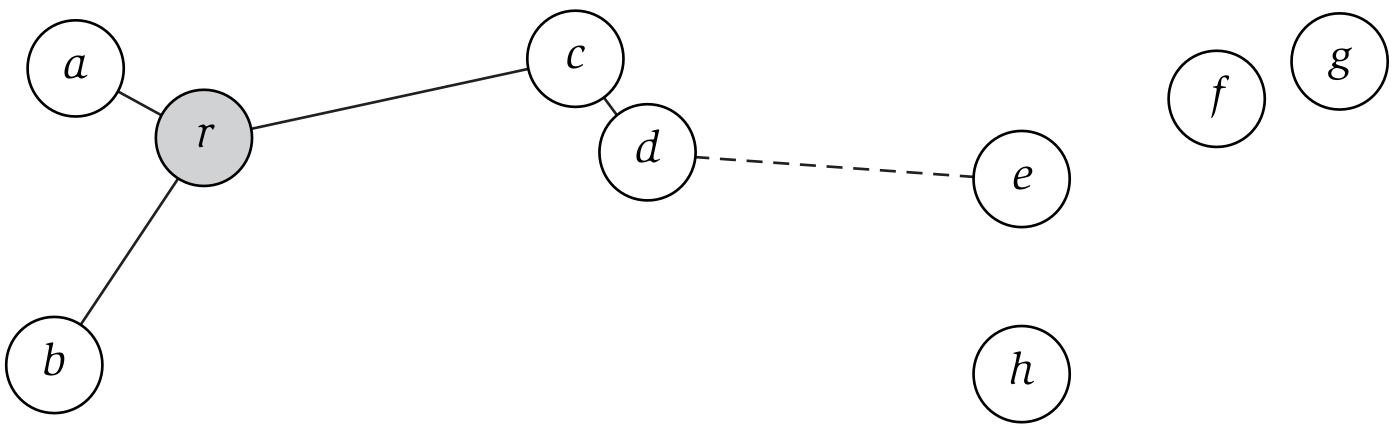
\includegraphics[width=0.7\linewidth]{img/execucao-prim}
	\end{figure}
	

	\begin{itemize}
		\item $r$ é o vértice raiz da busca.
		\item Arestas adicionadas: $\{r, a\}; \{r, b\}; \{r, c\}; \{c, d\}$.
		\item Algoritmo só adiciona arestas que farão parte da \textit{AGM}.
		\begin{itemize}
			\item Sempre escolhe a aresta de menor custo que liga a árvore já construída com algum vértice ainda desconectado.
		\end{itemize}
	\end{itemize}
\end{frame}



\begin{frame}{Algoritmo de Prim}
	\framesubtitle{Complexidade}
	
	\begin{itemize}
		\item A operação \texttt{extract-min} é executada $n$ vezes.
		\item O laço interno totaliza $m$ passos quando utilizada uma lista de adj.
		\begin{itemize}
			\item \texttt{update} é executado $m$ vezes no pior caso.
		\end{itemize}
		
		\item O laço interno totaliza $n^2$ passos quando utilizada uma matriz de adj.
		\begin{itemize}
			\item \texttt{update} é executado $n^2$ vezes no pior caso.
		\end{itemize}
	\end{itemize}

	\begin{table}
		\begin{tabular}{l|ll}
			& \textbf{matriz de adj.} & \textbf{lista de adj.} \\
			\hline
			\textbf{UnorderedPQ} & $O(n^2)$ & $O(n^2)$ \\
			\textbf{OrderedPQ} & $O(n^3)$ & $O(n^2)$ \\
			\textbf{BinaryHeap} & $O(n^2 \log n)$ & $O(m \log n)$ \\
		\end{tabular}
	\end{table}
\end{frame}



\begin{frame}{Exercício}
	\framesubtitle{Árvore geradora mínima}
	
	\begin{enumerate}
		\item Crie um programa que leia a especificação de um grafo e calcule a árvore geradora mínima, utilizando um dos algoritmos discutidos em aula. Aplique seu programa para determinar a árvore geradora mínima entre as cidades da região do Alto Vale do Itajaí.
	\end{enumerate}
\end{frame}


\frame{
	\frametitle{Referências}	
	\setlength{\bibsep}{8pt plus 0.3ex}
	\fontsize{10pt}{10}\selectfont
	\bibliographystyle{apalike}
	\bibliography{../referencias}
}

\end{document}